%%
%% This is file `sample-sigconf.tex',
%% generated with the docstrip utility.
%%
%% The original source files were:
%%
%% samples.dtx  (with options: `sigconf')
%% 
%% IMPORTANT NOTICE:
%% 
%% For the copyright see the source file.
%% 
%% Any modified versions of this file must be renamed
%% with new filenames distinct from sample-sigconf.tex.
%% 
%% For distribution of the original source see the terms
%% for copying and modification in the file samples.dtx.
%% 
%% This generated file may be distributed as long as the
%% original source files, as listed above, are part of the
%% same distribution. (The sources need not necessarily be
%% in the same archive or directory.)
%%
%% The first command in your LaTeX source must be the \documentclass command.
\documentclass[sigconf,review]{acmart}

\usepackage{listings}
\usepackage{tabularx}
\usepackage{cleveref}
\usepackage{xspace}
\usepackage{xcolor}

\newcommand{\logchunks}{\emph{LogChunks}\xspace}

%%
%% \BibTeX command to typeset BibTeX logo in the docs
\AtBeginDocument{%
  \providecommand\BibTeX{{%
    \normalfont B\kern-0.5em{\scshape i\kern-0.25em b}\kern-0.8em\TeX}}}

%% Rights management information.  This information is sent to you
%% when you complete the rights form.  These commands have SAMPLE
%% values in them; it is your responsibility as an author to replace
%% the commands and values with those provided to you when you
%% complete the rights form.
\copyrightyear{2020} 
\acmYear{2020} 
\setcopyright{acmlicensed}
\acmConference[MSR '20]{17th International Conference on Mining Software Repositories}{October 5--6, 2020}{Seoul, Republic of Korea}
\acmBooktitle{17th International Conference on Mining Software Repositories (MSR '20), October 5--6, 2020, Seoul, Republic of Korea}
\acmPrice{15.00}
\acmDOI{10.1145/3379597.3387485}
\acmISBN{978-1-4503-7517-7/20/05}



%%
%% Submission ID.
%% Use this when submitting an article to a sponsored event. You'll
%% receive a unique submission ID from the organizers
%% of the event, and this ID should be used as the parameter to this command.
%%\acmSubmissionID{123-A56-BU3}

%%
%% The majority of ACM publications use numbered citations and
%% references.  The command \citestyle{authoryear} switches to the
%% "author year" style.
%%
%% If you are preparing content for an event
%% sponsored by ACM SIGGRAPH, you must use the "author year" style of
%% citations and references.
%% Uncommenting
%% the next command will enable that style.
%%\citestyle{acmauthoryear}

%%
%% end of the preamble, start of the body of the document source.
\begin{document}

%%
%% The "title" command has an optional parameter,
%% allowing the author to define a "short title" to be used in page headers.
\title{LogChunks: A Data Set for Build Log Analysis}

\author{Carolin E. Brandt, Annibale Panichella, Andy Zaidman, Moritz Beller}
\email{{c.e.brandt, a.panichella, a.e.zaidman, m.m.beller}@tudelft.nl}
\affiliation{
  \institution{Delft University of Technology}
  \country{The Netherlands}
}

%%
%% By default, the full list of authors will be used in the page
%% headers. Often, this list is too long, and will overlap
%% other information printed in the page headers. This command allows
%% the author to define a more concise list
%% of authors' names for this purpose.
\renewcommand{\shortauthors}{Brandt, et al.}

%%
%% The abstract is a short summary of the work to be presented in the
%% article.
\begin{abstract}
Build logs are textual by-products that a software build process
creates, often as part of its Continuous Integration (CI)
pipeline. Build logs are a paramount source of information for
developers when debugging into and understanding a build
failure. Recently, attempts to partly automate this time-consuming,
purely manual activity have come up, such as rule- or
information-retrieval-based techniques.

We believe that having a common data set to compare
different build log analysis techniques will advance the research
area. It will ultimately increase our understanding of CI build
failures. In this paper, we present \logchunks, a collection of 797
annotated Travis CI build logs from 80 GitHub repositories in 29
programming languages. For each build log, \logchunks contains a
manually labeled log part (chunk) describing why the build failed. We
externally validated the data set with the developers who caused the
original build failure.

The width and depth of the \logchunks data set are intended to
make it the default benchmark for automated build log analysis
techniques.
\end{abstract}

%%
%% The code below is generated by the tool at http://dl.acm.org/ccs.cfm.
%% Please copy and paste the code instead of the example below.
%%
%\begin{CCSXML}
%<ccs2012>
% <concept>
%  <concept_id>10010520.10010553.10010562</concept_id>
%  <concept_desc>Computer systems organization~Embedded systems</concept_desc>
%  <concept_significance>500</concept_significance>
% </concept>
% <concept>
%  <concept_id>10010520.10010575.10010755</concept_id>
%  <concept_desc>Computer systems organization~Redundancy</concept_desc>
%  <concept_significance>300</concept_significance>
% </concept>
% <concept>
%  <concept_id>10010520.10010553.10010554</concept_id>
%  <concept_desc>Computer systems organization~Robotics</concept_desc>
%  <concept_significance>100</concept_significance>
% </concept>
% <concept>
%  <concept_id>10003033.10003083.10003095</concept_id>
%  <concept_desc>Networks~Network reliability</concept_desc>
%  <concept_significance>100</concept_significance>
% </concept>
%</ccs2012>
%\end{CCSXML}
%
%\ccsdesc[500]{Computer systems organization~Embedded systems}
%\ccsdesc[300]{Computer systems organization~Redundancy}
%\ccsdesc{Computer systems organization~Robotics}
%\ccsdesc[100]{Networks~Network reliability}

%%
%% Keywords. The author(s) should pick words that accurately describe
%% the work being presented. Separate the keywords with commas.
\keywords{CI, Build Log Analysis, Build Failure, Chunk Retrieval}

%%
%% This command processes the author and affiliation and title
%% information and builds the first part of the formatted document.
\maketitle

\section{Introduction}
Continuous Integration (CI) has become a common practice in software
engineering~\cite{hilton2016usage}.  Many software projects use
CI~\cite{hilton2016usage,staahl2014modeling,beller2017oops} to detect
bugs early~\cite{vasilescu2015quality,duvall2007continuous}, improve
developer productivity~\cite{miller2008hundred,hilton2016usage} and
communication~\cite{downs2012ambient}.  CI builds produce logs which
report results of various sub-steps within the build.  These build logs
contain a lot of valuable information for developers and researchers---for example, descriptions of compile errors, linter warnings or failed
tests~\cite{beller2017oops,seo2014programmers,vassallo2017a-tale}.

However, build logs can be verbose and large---sometimes in excess of
50 MB of ASCII text ~\cite{beller2017oops}---making them inadequate
for direct human consumption. Therefore, to support developers and
researchers in efficiently making use of the information within build
logs, we must at least semi-automatically retrieve the chunks of the
log that describe the targeted information.

There are different techniques to retrieve information chunks from CI
build logs. Beller et al. use a rule-based system of regular
expressions to analyze logs from Travis CI~\cite{beller2017oops}.
Such regular expressions are developed by looking at exemplary build
logs.  Vassallo et al.\ wrote a custom parser to gather information
for build repair hints~\cite{vassallo2018un-break}.  Recently, Amar et
al.\ reduced the number of lines for a developer to inspect by
creating a diff between logs from failed and successful
builds~\cite{amar2019mining}.

These approaches have various strengths and weaknesses: Regular
expressions are exact, but tedious and error-prone to
maintain~\cite{michael2019regexes}.  Custom parsers are powerful
though fragile in light of changes in the log structure. Diffing
between failed and successful logs can reduce the information to be
processed, but is at best semi-automatic~\cite{amar2019mining}.

At the moment, there is only anecdotal evidence on the performance of
these techniques, and when a technique should be preferred over its
alternatives.  In fact, there is no data set available to support the
creation of such a benchmark for build log analysis techniques.
Following Sim et al., a benchmark gives us the chance to ``increase
the scientific maturity of the area''~\cite{sim2003using} of build log
analysis by evaluating and comparing research contributions.

Thus, in this paper, we present
\logchunks~\cite{brandt_carolin_2020_3632351},\footnote{\logchunks is
  openly available on Zenodo: \url{https://zenodo.org/record/3632351}} a
collection of 797 labeled Travis CI build logs from 80 highly popular GitHub
repositories in 29 programming languages with  we
manually labeled the chunk describing why the build failed.  The data
set also provides keywords the authors would use to search for the
labeled log chunk and categorizes the log chunks according to their
format within the log.


\begin{figure*}[tbp]
	\centering
	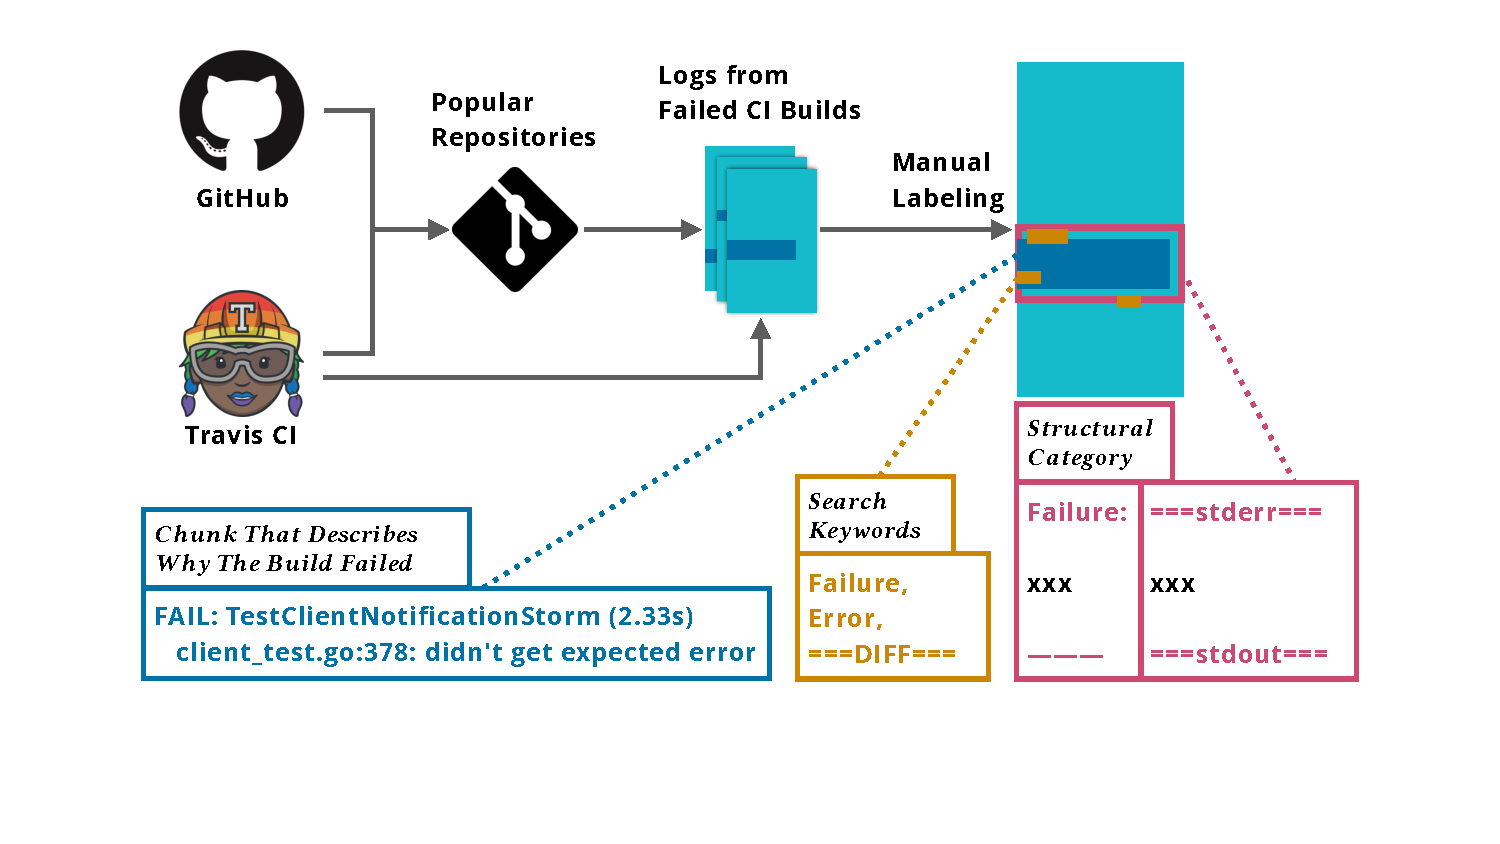
\includegraphics[width=1.35\columnwidth, trim={2cm 2cm 2cm 0.5cm}, clip]{overview.pdf}
	\caption{Overview of \logchunks}
	\label{fig:lc-overview}
\end{figure*}

\section{Creating \logchunks}
This section presents how we gathered the logs and our manual labeling process.
\label{sec:data-collection}

\subsection{Log Collection}
In this section, we describe along the overview in
\Cref{fig:lc-overview} how we created \logchunks. All steps are
automatized as Ruby scripts\footnote{Data collection scripts and their original
parameterization are included in the data set.} and highly configurable.

\paragraph{Repository Sampling}
We target mature GitHub repositories that are using Travis CI\@.
To avoid personal and toy projects we select popular projects based
on the number of users that starred a project~\cite{kalliamvakou2016depth}.
We query \emph{GHTorrent}~\cite{gousios2013ghtorrent} for the
most popular languages on GitHub, and subsequently, the most popular
repositories for a given language.

For \logchunks, we queried GHTorrent from 2018-04-01 for the three
most popular repositories of each of the 30 most popular languages
to cover a broad range of development languages.
Among the resulting repositories are, for example, \texttt{git/git},
\texttt{Microsoft/TypeScript} and \texttt{jwilm/alacritty}.

\paragraph{Build Sampling}
To sample builds for \logchunks we keep the ten most recent builds of the status 
\emph{failed}~\cite{travis2009buildstatus}. We check up to 1,000 builds per 
repository to ensure predictable termination of the log collection.
\paragraph{Log Sampling}
Travis CI builds comprise a number of jobs that actualize a build
process in different environments. Hence, the outcome from different
jobs might be different. For each build in \logchunks, we download the log of the
first job that has the same state as the overall build.

We inspected the collected
build logs and discarded logs from three repositories.  One had only
one failed build, two others had empty build logs on Travis CI\@.  In
total, we collected 797 logs from 80 repositories spanning 29
languages.

\subsection{Manual Labeling}
\label{sec:labeling-process}
After collecting build logs, the first author manually labeled which
text chunk describes why the build failed. Following that, she
assigned search keywords and structural categories to each log chunk.

\paragraph{Chunk That Describes Why The Build Failed}
For each repository, the labeler skimmed through the build logs and copied out the first occurrence of a description why the build failed.
She preserved whitespaces and special characters, as these might be crucial to detect the targeted substring.
To support learning of regular expressions identifying the labeled substrings the labeler aimed to start and end the labeled substring at consistent locations around the fault description.

\paragraph{Search Keywords}
To extract the search keywords, we considered the \texttt{Chunk} and ten lines above and below.
The labeler's task was to note down three strings they would search for (``grep'') to find this failure description.
The strings should appear in or around the \texttt{Chunk} and are case-sensitive.
We made no limitations on the search string; particularly, spaces are allowed.

\paragraph{Structural Category}
To label the \emph{structural categories} we presented the \texttt{Chunk} and the surrounding context to the labeler for all logs from a repository.
We asked the labeler to assign numerical categories according to whether the \texttt{Chunk} had the same structural representation.


\subsection{Validation}
\label{sec:validation}

We validated our collected data points in an iterative fashion. First,
we performed an initial inter-rater reliability study with the second author of this paper. Our learnings from this
initial internal study are that  1) it is important and difficult to
adequately communicate all decisions and assumptions on how to and which data to
label and 2) there can be different legitimate viewpoints on
which log chunk constitute the cardinal error and which keywords best to use. These learning informed the design of a second, larger cross-validation study for which we contacted over 200 developers.

In our second validation, we sent out emails to the original
developers whose commits triggered the builds represented in
\logchunks and asked them whether the log chunk we labeled
actually describes why the build failed.  This section describes our
survey and discusses our results.

\paragraph{Method}
Using the Travis API, we collected the commit information for each build represented in \logchunks.
We grouped all commits triggered by one developer and sent out an email to them. 
It included links to the corresponding commits, the build overview and the log file.
We asked the developers to fill out a short form in case our extraction was not correct.
In the survey, we asked the developer to paste in the log part actually describing the failure reason or describe in their own words why our original extraction was incorrect.

\paragraph{Results}
In total, from 2019-10-15 to 2019-10-17, we sent out emails to 246 developers. Of these, 32 could
not be delivered. We performed the sending out in three batches and used the first author's academic email address as the sender. All emails were specific to each recipient. We only sent one mail per recipient. We received answers from 61 developers, corresponding to
144 build logs with a response rate of 24.8\%. Compared to typical response rates to cold calling known from Software Engineering~\cite{smith2013improving}, this is very high. We believe that our personalization and the ease of use for the participant are the main reasons for this---simply clicking on a link to confirm or refute an answer is enough, there is no need to craft an answer. Indeed, we only received seven replies from developers along the lines of ``done.''

Of the 144 answers, 118 initially indicated that our extraction was correct.
We manually inspected the 26 negative answers and found that some stated that the proposed extraction did not show the whole description of why the build failed.
This was because we chose to trim long chunks to keep the mails readable, and not a fault in our extraction per se. After adjusting for these answers, only 12 answers remained that stated that our labeled log chunk was not correct. This validates our data set with an externally validated consensus on 94.4\% of the extracted data.

\paragraph{Discussion}
We believe that our developer survey highly strengthens the trust in
the validity of the labeled log chunks.  The study received answers
for about 18\% of the data in \logchunks.  After manual
correction, 91\% of the received answers indicated our labeled chunks
were accurate.  One possible threat regarding the high number of
correct answers is that, since we show the error message we extracted,
it might be operationally easier for developers to validate it, rather
than search for it in a long log file. To alleviate this problem, we
made it as easy to confirm as to reject an extracted log chunk. We
only ask for more details (the correct log chunk) in a second step.

One of our 12 incorrect extractions only showed a warning and the
developer proposed to also include the line stating that warnings are
treated as errors. In others, we labeled the error message of an error
that was later ignored.

\begin{table*}[htbp]
\centering
\begin{tabularx}{\textwidth}{@{}lXlX@{}}
  \toprule
  Data & Description & Unit & Example \\
  \midrule
  Log & Relative path to the input build log & Unique Path & \tt{C/php@php-src/failed/529279089.log} \\
  Chunk & Log chunk that describes why the build failed & String & \tt{001+ ** ERROR: process timed out **\newline
001- OK.\newline
========DONE========\newline
FAIL Bug \#60120 (proc\_open hangs)} \\ 
  Keywords & Keywords the authors would use to search for and find the log chunk & List of Strings & \tt{ERROR, FAIL, DIFF} \\ 
  Category & Categorization of the structural representation of the log chunk within the build log & Integer & \tt{0}\\
  \bottomrule
\end{tabularx}
\caption{Exemplary, complete data excerpt from \logchunks for a failed build in \tt{php@php-src}.}
\label{tab:data-in-example}
\vspace{-0.5cm}
\end{table*}

\section{Data Schema}
\label{sec:data-schema}

This section presents the internal structure and data schema of
\logchunks. In principle, \logchunks comprises automatically
retrieved and manually labeled and cross-validated logs.

\logchunks comprises information on 797 build logs, which are organized in folders for each language and repository.
For each repository, \logchunks has about 10 \texttt{Examples}. Every repository folder contains the full log files for the build status `failed' in plain text.

The folder \texttt{build-failure-reason} contains the manually labeled
data of \logchunks, one XML file for each repository: \\
\texttt{\textless repository\_owner\textgreater @\textless
  repository\_name\textgreater.xml}.  \Cref{tab:data-in-example} gives
an overview of the data within these XML files on the example of one
build from \texttt{php@php-src}. The remainder of this section defines
in more detail the data embedded in the XML files, that is, the
labeled log chunk, search keywords and structural categories. Data from the developer validation study is in the file \texttt{developer-crossvalidation.csv}, the build id can be used as a unique identifier to match it with the other data.

\paragraph{Chunk That Describes Why The Build Failed}
The \texttt{Chunk} is the substring of the build log that describes why the build failed.
This can, for example, be the failing test case or a compiler error.
In cases where the reason \emph{why} the build failed is contained in a log file external to the main build log, the \texttt{Chunk} includes only the fact \emph{that} the build failed, for example ``\texttt{The command "test/run !" exited with 1.}''
In \Cref{tab:data-in-example}, the \texttt{Chunk} describes a failing test in which the tested process timed out.

\paragraph{Search Keywords}
The \texttt{Keywords} contain a list of one to three freely chosen search strings appearing within the \texttt{Chunk} or in the area around it in the build log.
We selected keywords the authors would use to search for the log \texttt{Chunk}, as we found them repeatedly next to failure describing chunks while analyzing about 800 build logs manually.
Some keywords from \logchunks are  ``\texttt{Error}'', ``\texttt{=DIFF=}'', ``\texttt{ERR!}'', or the keywords shown in \Cref{tab:data-in-example}.

\paragraph{Structural Category}
For each repository, we assign \emph{structural categories} to the \texttt{Chunk}s.
The structural category compares how \texttt{Chunk}s are represented within the build log.
Build tools highlight their error messages with markings, e.g.\ starting each line with ``\texttt{ERROR}'' or surrounding special characters.
Two chunks fall into the same structural categories if they are surrounded by the same markings.
Listing \ref{lst:same-category} presents a log chunk from the same category as the log chunk from \Cref{tab:data-in-example}.
In comparison to that, Listing \ref{lst:different-category} presents a log chunk which is formatted differently within the log file.
For each repository, the structural categories are represented as integers, starting at 0 and increased with the next appearing category in chronological build order.

\lstset{
  language=XML,
  basicstyle=\footnotesize,
  morekeywords={Examples, Example, Log, Keywords, Category, Chunk},
  postbreak=\mbox{\textcolor{cyan}{$\hookrightarrow$}\space},
	frame=single,
	escapeinside=**
}
\begin{figure}[tbp]
	\centering
\begin{lstlisting}[breaklines=true]
========DIFF========
*{\color{cyan}-=-=-=-=-=-}*
005+     Parameter #1 [<optional> $flags]
005-     Parameter #1 [<optional> $ar_flags]
========DONE========
FAIL Bug#71412 ArrayIterator reflection 
*{\color{cyan}-=-=-=-=-=-}*
TEST 9895/13942 [2/2 test workers running]
\end{lstlisting}
\vspace{-0.3cm}
	\caption{Log chunk from the \emph{same} structural category as the log chunk presented in \Cref{tab:data-in-example}. We inserted the special marker ``{\color{cyan}-=-=-=-=-=-}'' to separate the log chunk from its context.}
	\label{lst:same-category}
\end{figure}

\begin{figure}[tbp]
	\centering
\begin{lstlisting}[breaklines=true]
[0K$ ./sapi/cli/php run-tests.php -P ...
*{\color{cyan}-=-=-=-=-=-}*
Illegal switch 'j' specified!
*{\color{cyan}-=-=-=-=-=-}*
Synopsis:
\end{lstlisting}
\vspace{-0.3cm}
	\caption{Log chunk from a \emph{different} structural category than the log chunk presented in \Cref{tab:data-in-example}.}
  %, ``{\color{cyan}-=-=-=-=-=-}'' separates the log chunk from the context}
	\label{lst:different-category}
        \vspace{-0.3cm}
\end{figure}

\section{Potential Use Cases}

\logchunks can be the basis for a range of further studies:

\paragraph{Benchmarking Build Log Analysis Techniques}
\logchunks originated from the first author's Master's Thesis in which she compared three different log chunk retrieval techniques. %\todo{cite journal paper (or preprint?)}.
\logchunks can be a benchmark to evaluate other build log analysis techniques.
For example, one can use the data set to investigate how reliably the diff-based approach of Amar et al.~\cite{amar2019mining} retrieves build failure reasons.

\paragraph{Support Build Log Classification Algorithms}
Various researchers examine why CI builds fail and use build logs as a data source~\cite{seo2014programmers,vassallo2017a-tale}.
They typically write custom parsers and classifiers to categorize builds according to why a build failed.
The manually labeled chunk can help researchers locate the source for their classification algorithms and cross-validate their data.

\paragraph{Research on Build Logs}
The data from \logchunks can support research around the topic of build logs such as how developers use keywords to retrieve information about build failures from logs or how they discuss failures of CI builds within pull requests~\cite{cassee2019silent}.

\paragraph{Automatic Processing of Build Results}
\logchunks enables researchers to train algorithms that retrieve build failure
descriptions from build logs. It can provide the basis for further automatic
on-ward processing of the retrieved log chunks.

\section{Related Data Sets}
\label{sec:related-data-sets}
This section presents existing data sets of CI build logs and how
\logchunks differs from them.

\subsection{TravisTorrent}
\emph{TravisTorrent}~\cite{beller2017travistorrent} collects a broad
range of metadata about Travis CI builds\@.  It combines data
accessible through the public Travis CI and GitHub APIs and through
GHTorrent~\cite{gousios2013ghtorrent}. Similar to \logchunks, among the
metadata are the failing test cases. However, TravisTorrent obtained
these through a manually developed parser, which only supports
specific Ruby test runners and Java Maven or JUnit logs. Anecdotally,
many of the failing tests are at least incomplete and lack
validation. By contrast, \logchunks provides manually labeled
and two-fold cross-validated data of why builds failed, not only for
failing tests like TravisTorrent, but for all possible build-failing
errors.

\subsection{LogHub}
\emph{LogHub}~\cite{zhu2019tools} is a collection of a wide range of system log data sets.
It is the basis for various studies that compare different approaches to parse unstructured system log messages into structured data for further analysis. \logchunks is situated in a different area, build log analysis, which tend to be semi-structured, and could play a similar role to \emph{LogHub} in its area: 
empower research with a benchmark to compare different build log analysis techniques.

\section{Future Extensions to \logchunks}

In this section, we describe current limitations and future improvements of \logchunks and extensions we are planning.

\paragraph{Chunk as One Consecutive Substring}
The \texttt{Chunk} contains only one continuous substring of the log text.
The reason a build failed could be described at multiple locations within the log.
We propose to extend \logchunks to contain multiple substrings of the log text.

\paragraph{Include More Repositories and Logs}
\logchunks encompasses a range of repositories from various main development languages, though only 10 logs from each repository.
%This stems from the high effort necessary for the manual data labeling process.
Including more logs and repositories will strengthen \logchunks as the go-to benchmark.

\paragraph{Classification of the Build Failure Cause}
Our data set contains no further classification according to the cause of the failure, such as due to tests, compilation or linter errors.
As researchers are investigating why CI builds fail, a useful extension is to annotate cause of the build failure for each log.

\paragraph{Other Information Chunks}
Build log analysis is not limited to the chunk that describes why a build failed.
\logchunks can be extended with labels for all information that is contained in the build log, such as descriptions of warnings, build infrastructure and more.

\paragraph{Validation of Search Keywords}
The keywords \logchunks provides are based on the experience of the authors gained from analyzing around 800 build logs.
Next, we propose to evaluate whether these keywords would also be used by developers to find the log chunk describing why a build failed.



\section{Summary}
\label{sec:conclusion}
In this paper, we introduce \logchunks, a cross-validated data
set encompassing 797 build logs from 80 projects using Travis CI\@.
For each log, we annotated the log chunk describing why the build
failed and provided keywords a developer would use to search for the
log chunk as well as a categorization of the log chunks according to
their format within the log. \logchunks advances the research
field of build log analysis by introducing a benchmark to rigorously
examine research contributions~\cite{sim2003using} and opening various
research possibilities that previously required tedious manual
classification.

%%
%% The acknowledgments section is defined using the "acks" environment
%% (and NOT an unnumbered section). This ensures the proper
%% identification of the section in the article metadata, and the
%% consistent spelling of the heading.

% \begin{acks}
% To Robert, for the bagels and explaining CMYK and color spaces.
% \end{acks}

%%
%% The next two lines define the bibliography style to be used, and
%% the bibliography file.
\bibliographystyle{ACM-Reference-Format}
\bibliography{paper}

%%
%% If your work has an appendix, this is the place to put it.
% \appendix

% \section{Research Methods}

% \subsection{Part One}


\end{document}
\endinput
%%
%% End of file `sample-sigconf.tex'.
